% A tervezett laboratóriumi tesztkörnyezet (6. fejezet). Fordítás: pdflatex labor.tex
\documentclass[tikz,border=4pt]{standalone}
\usepackage[utf8]{inputenc}
\usepackage[T1]{fontenc}
\usepackage{times}
\usetikzlibrary{positioning,arrows.meta,fit,backgrounds,calc}
\definecolor{det}{HTML}{1D294D}
\definecolor{detbg}{HTML}{E6ECF7}
\definecolor{red}{HTML}{9B2C2C}
\definecolor{redbg}{HTML}{FDE8E8}
\definecolor{llm}{HTML}{B7791F}
\definecolor{llmbg}{HTML}{FEEFCF}
\definecolor{dat}{HTML}{4A5568}
\definecolor{datbg}{HTML}{F3F4F7}
\begin{document}
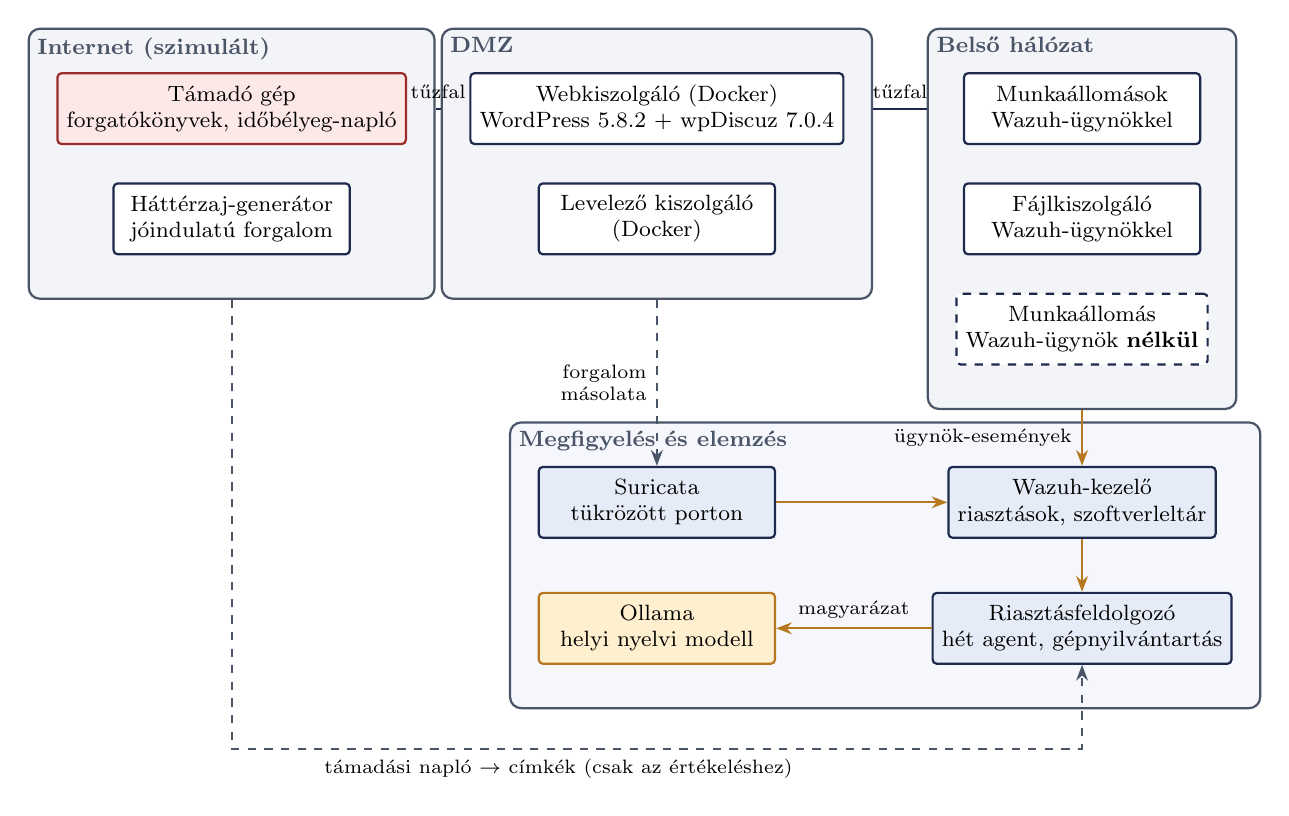
\begin{tikzpicture}[
  font=\footnotesize, node distance=4mm and 6mm,
  host/.style={draw=det, fill=white, thick, rounded corners=1.5pt, minimum width=30mm,
               minimum height=9mm, align=center},
  att/.style={host, draw=red, fill=redbg},
  mon/.style={host, fill=detbg},
  zone/.style={draw=dat, thick, rounded corners=4pt, fill=datbg, inner sep=3.5mm},
  zlabel/.style={font=\footnotesize\bfseries, text=dat, anchor=north west},
  net/.style={thick, draw=det},
  mir/.style={-{Stealth[length=2mm]}, thick, dashed, draw=dat},
  ev/.style={-{Stealth[length=2mm]}, thick, draw=llm},
]
% hálózati zónák (felső sor)
\node[att] (kali) at (0,0) {Támadó gép\\ forgatókönyvek, időbélyeg-napló};
\node[host] (noise) at (0,-14mm) {Háttérzaj-generátor\\ jóindulatú forgalom};
\node[host] (wp) at (54mm,0) {Webkiszolgáló (Docker)\\ WordPress 5.8.2 + wpDiscuz 7.0.4};
\node[host] (mail) at (54mm,-14mm) {Levelező kiszolgáló\\ (Docker)};
\node[host] (ws1) at (108mm,0) {Munkaállomások\\ Wazuh-ügynökkel};
\node[host] (fs) at (108mm,-14mm) {Fájlkiszolgáló\\ Wazuh-ügynökkel};
\node[host, dashed] (ws2) at (108mm,-28mm) {Munkaállomás\\ Wazuh-ügynök \textbf{nélkül}};
% megfigyelés és elemzés (alsó sorok)
\node[mon] (sur) at (54mm,-50mm) {Suricata\\ tükrözött porton};
\node[mon] (wm) at (108mm,-50mm) {Wazuh-kezelő\\ riasztások, szoftverleltár};
\node[mon] (aa) at (108mm,-66mm) {Riasztásfeldolgozó\\ hét agent, gépnyilvántartás};
\node[host, draw=llm, fill=llmbg] (ol) at (54mm,-66mm) {Ollama\\ helyi nyelvi modell};
% zónák
\begin{scope}[on background layer]
\node[zone, fit=(kali)(noise), inner ysep=5.5mm] (zi) {};
\node[zone, fit=(wp)(mail), inner ysep=5.5mm] (zd) {};
\node[zone, fit=(ws1)(fs)(ws2), inner ysep=5.5mm] (zb) {};
\node[zone, fit=(sur)(wm)(aa)(ol), inner ysep=5.5mm, fill=detbg!40] (zm) {};
\end{scope}
\node[zlabel] at (zi.north west) {Internet (szimulált)};
\node[zlabel] at (zd.north west) {DMZ};
\node[zlabel] at (zb.north west) {Belső hálózat};
\node[zlabel] at (zm.north west) {Megfigyelés és elemzés};
% kapcsolatok
\draw[net] (zi.east |- kali) -- node[above, font=\scriptsize]{tűzfal} (zd.west |- wp);
\draw[net] (zd.east |- wp) -- node[above, font=\scriptsize]{tűzfal} (zb.west |- ws1);
\draw[mir] (zd.south) -- node[left, font=\scriptsize, align=right]{forgalom\\ másolata} (sur.north);
\draw[ev] (zb.south) -- node[left, font=\scriptsize]{ügynök-események} (wm.north);
\draw[ev] (sur) -- (wm);
\draw[ev] (wm) -- (aa);
\draw[ev] (aa) -- node[above, font=\scriptsize]{magyarázat} (ol);
\draw[mir] (zi.south) |- node[pos=0.75, below, font=\scriptsize]{támadási napló $\rightarrow$ címkék (csak az értékeléshez)} ($(zm.south)+(0,-5mm)$) -| (aa.south);
\end{tikzpicture}
\end{document}
